%! Author = joels
%! Date = 10/01/2022

\section{GoF Patterns}
%Creational
\subsection{Factory Method (Creational)}
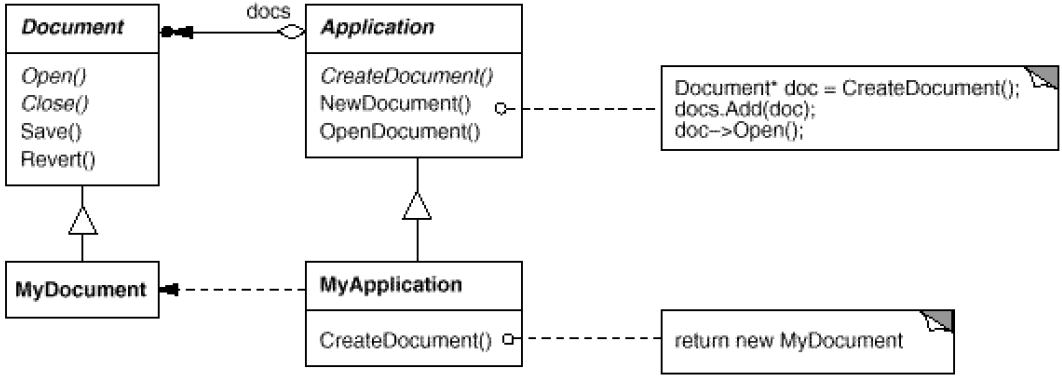
\includegraphics[width=\linewidth]{/factory_method}
\subsubsection{Beschreibung}
Define an interface for creating an object, but let the subclass decide which class to instantiate. Factory Method lets a class defer instantiation to subclasses.
\subsubsection{Vorteile}
\begin{itemize}[topsep=0pt]
    \itemsep -0.4em
    \item Verhindert eine Kopplung zwischen dem Creator und dem konkretem produkt
    \item Single Responsibility Principle: Der Product Creation Code kann einfach herumgeschoben werden $\rightarrow$ Macht den Support einfacher
    \item Open/Closed Principle: Es können neue Produkt-Typen hinzugefügt werden, ohne den Client Code zu zerstören
\end{itemize}
\subsubsection{Nachteile}
\begin{itemize}[topsep=0pt]
    \itemsep -0.4em
    \item Code kann komplizierter werden, weil viele Sub-Klassen erstellt werden müssen
\end{itemize}
\subsubsection{Eigene Notizen}
\textbf{Intent:} return new MyDocument
\textbf{Identifikation:} Haben eine Creation-Methode, die Objekte von konkreten Klassen erstellen, diese aber als Objekte von abstrakten Klassen oder Interfaces zurückgibt.

\subsection{Abstract Factory (Creational)}
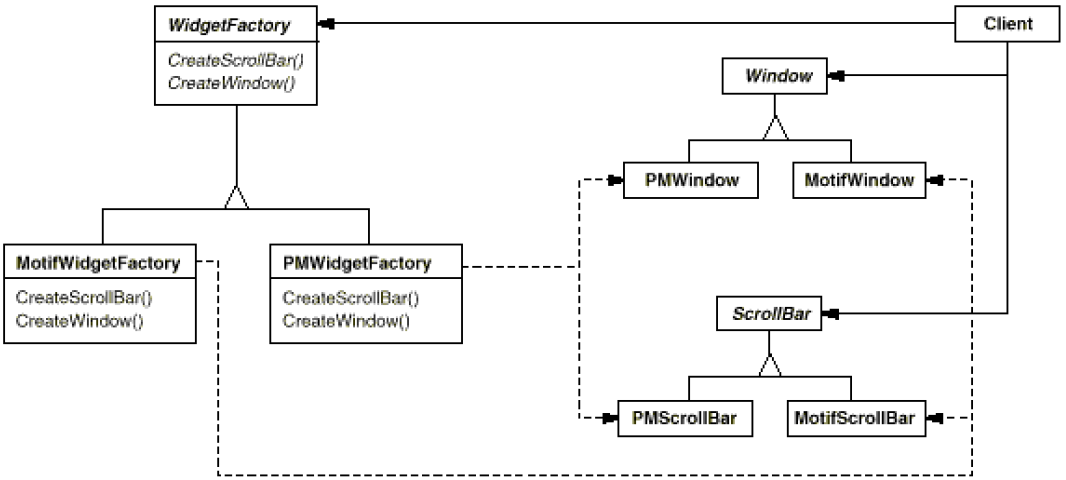
\includegraphics[width=\linewidth]{/abstract_factory}
\subsubsection{Beschreibung}
Provide an interface for creating families of related or dependant objects without specifying their concrete classes.
\subsubsection{Vorteile}
\begin{itemize}[topsep=0pt]
    \itemsep -0.4em
    \item Man kann sicher sein, dass die Produkte einer Factory miteinander kompatibel sind
    \item Vermeidet enge Kopplung zwischen konkreten Produkten und Client Code
    \item Single Responsibility Principle: Der Product Creation Code kann einfach herumgeschoben werden $\rightarrow$ Macht den Support einfacher
    \item Open/Close Principle: Es können neue Varianten hinzugefügt werden, ohne existierenden Code zu zerstören
\end{itemize}
\subsubsection{Nachteile}
\begin{itemize}[topsep=0pt]
    \itemsep -0.4em
    \item Der Code kann komplizierter werden, als er sein sollte, da mit diesem Pattern viele neue Interfaces und Klassen erstellt werden
\end{itemize}
\subsubsection{Eigene Notizen}
\textbf{Identifikation:} Methoden, die ein Factory-Objekt zurückgeben, welches dann verwendet wird um spezifische Sub-Komponenten zu erstellen\\
\textbf{Factory Method:} Verwendet eigentlich immer das Pattern Factory Method (grössere Variante davon)\\
\textbf{Beispiel 1:} Unterschiedliche Buttons für Windows und MacOS. Dabei sind Windows \& MacOS die factories\\
\textbf{Beispiel 2:} Window Manager in einem Linux System (je nachdem, ob Gnome oder KDE installiert ist)

\subsection{Prototype (Creational)}
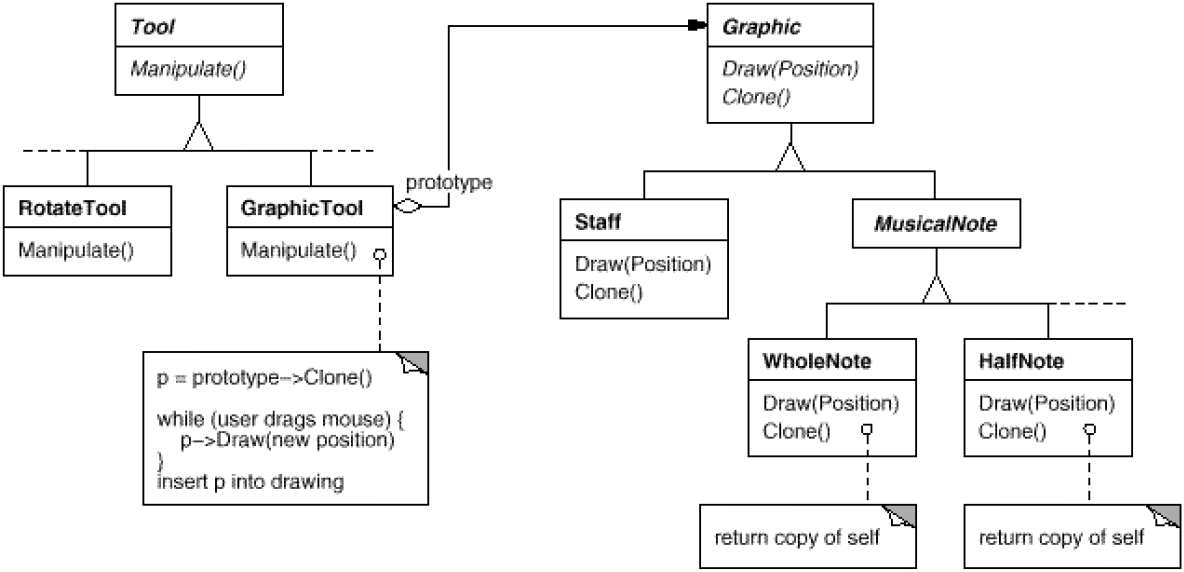
\includegraphics[width=\linewidth]{/prototype}
\subsubsection{Beschreibung}
Specify the kinds of objects to create using a prototypical instance, and create new objects by copying this prototype.
\subsubsection{Vorteile}
\begin{itemize}[topsep=0pt]
    \itemsep -0.4em
    \item Objekte können geklont werden, ohne Kompplung zu dessen konkreter Klasse
    \item Wiederholte Initialisierung kann durch das Klonen vermiedenw erden
    \item Komplexe Objekte können bequemer erstellt werden
    \item Alternative von Vererbung beim Umgang mit Voreinstellungen für komplexe Objekte
\end{itemize}
\subsubsection{Nachteile}
\begin{itemize}[topsep=0pt]
    \itemsep -0.4em
    \item Sehr tricky Objekte mit zirkularen Referenzen zu klonen
\end{itemize}
\subsubsection{Eigene Notizen}
\textbf{Identifikation:} Hat eine clone(), oder copy()-Methode\\
\textbf{Beispiel:} Musik-Noten darstellen: Die existierenden Noten in einen Manager (Pool) laden und diese jeweils bei Gebrauch klonen\\
\textbf{Einsetzen:} Ist eine möglichkeit, wenn Daten von externen Quellen sehr ineffizient geladen werden (Clone erstellen um effizienz zu steigern)

%Structural
\subsection{Composite (Structural)}
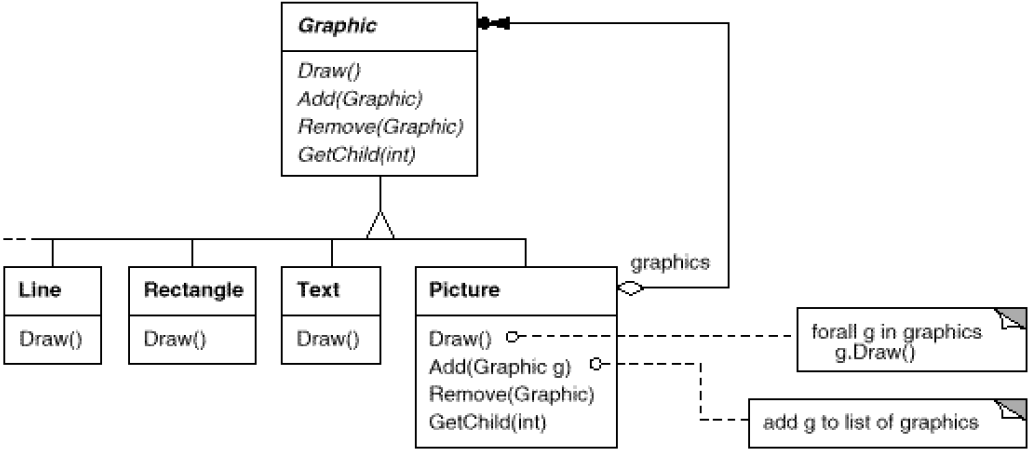
\includegraphics[width=\linewidth]{/composite}
\subsubsection{Beschreibung}
Compose objects into tree structures to represent part-whole hierarchies. Composite lets clients treat individual objects and compositions of objects uniformly.
\subsubsection{Vorteile}
\begin{itemize}[topsep=0pt]
    \itemsep -0.4em
    \item Bequemer um mit komplexen Baumstrukturen zu arbeiten. Verwende Polymoprhismus und Rekursion zum Vorteil
    \item Open/Closed Principle Es können neue Element-Typen hinzugefügt werden, ohne den existierenden Code zu zerstören
\end{itemize}
\subsubsection{Nachteile}
\begin{itemize}[topsep=0pt]
    \itemsep -0.4em
    \item Es kann schwierig sein, eine gemeinsame Schnittstelle anzubieten
\end{itemize}
\subsubsection{Eigene Notizen}
\textbf{Identifkation:} Haben Baum-Struktur und Klassen die Arbeit zu dessen Kinder delegieren

\subsection{Decorator (Structural)}
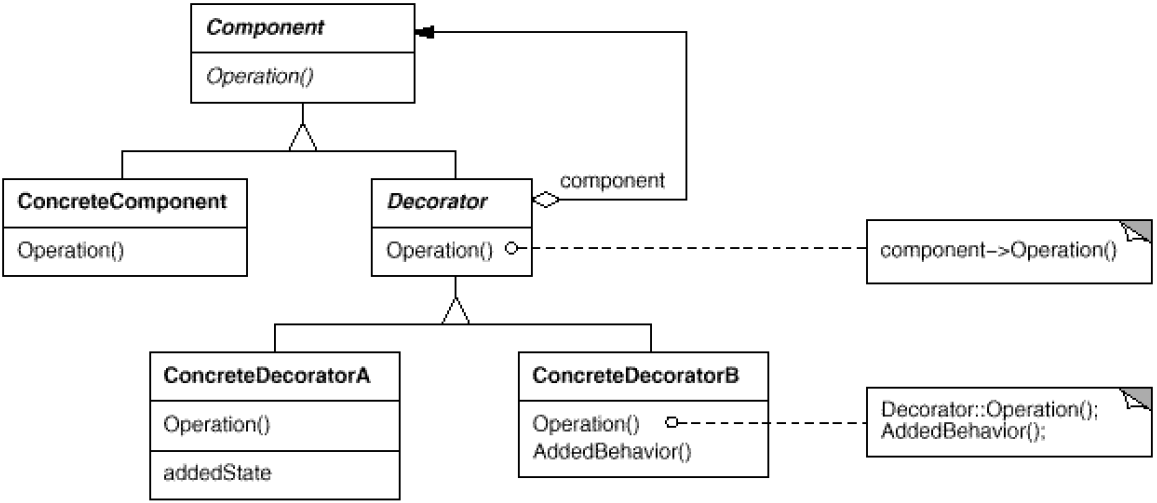
\includegraphics[width=\linewidth]{/decorator}
\subsubsection{Beschreibung}
Attach additional responsibilities to an object dynamically. Decorators provide a flexible alternative to subclassing for extending functionality.
\subsubsection{Vorteile}
\begin{itemize}[topsep=0pt]
    \itemsep -0.4em
    \item Das Verhalten eines Objekts kann erweitert werden, ohne Sub-Klassen zu erstellen
    \item Verantwortungen können zur Laufzeit einem Objekt hinzugefügt und entfernt werden
    \item Mehrere Verhalten können kombiniert werden, indem ein Objekt in mehrere Decorator gewrappt wird
    \item Single Responsibility Principle: Ein Monolith kann in mehrere kleine Klassen unterteilt werden
\end{itemize}
\subsubsection{Nachteile}
\begin{itemize}[topsep=0pt]
    \itemsep -0.4em
    \item Es ist schwer ein Wrapper vom Wrapper-Stack zu entfernen
    \item Es ist schwer ein Decorator so zu implementieren, dass die Reihenfolge keine Rolle spielt
    \item Der initiale Configuration Code von Layers kann ugly aussehen
\end{itemize}
\subsubsection{Eigene Notizen}
\textbf{Identifikation:} Hat Creation-Methode oder Konstruktur die Objekte der selben Klasse akzeptieren, wie die eigene Klasse\\
\textbf{Super:} Es wird viel mit dem super-Keyword gearbeitet

\subsection{Adapter (Structural)}
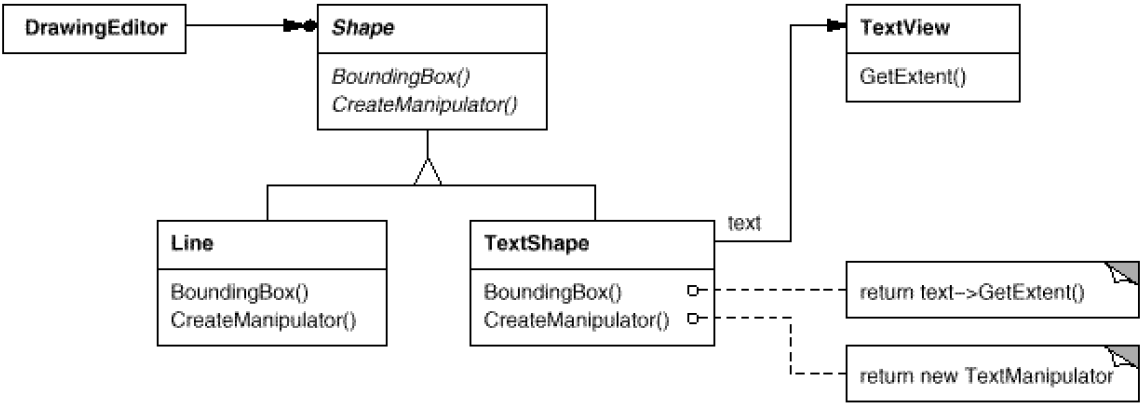
\includegraphics[width=\linewidth]{/adapter}
\subsubsection{Beschreibung}
Convert the interface of a class into another interface clients expect. Adapter lets classes work together that couldn't otherwise because of incompatible interfaces.
\subsubsection{Vorteile}
\begin{itemize}[topsep=0pt]
    \itemsep -0.4em
    \item Single Responsibility Principle: Das Interface oder Data Conversion Code kann von der Business Logik separiert werden
    \item Open/Closed Principle Es können neue Adapters hinzugefügt werden, ohne den Client Code zu zerstören
\end{itemize}
\subsubsection{Nachteile}
\begin{itemize}[topsep=0pt]
    \itemsep -0.4em
    \item Die Gesamt-Komplexität des Codes steigt, weil neue Interfaces und Klassen erstellt werden müssen
\end{itemize}
\subsubsection{Eigene Notizen}
\textbf{Identifikation:} Nehmen im Konstruktur eine Instanz eines anderen Types. Diese wird verwendet, um in Methoden die Methoden der Instanz auszuführen.\\
\textbf{Anwendung:} Erbe von dem was du sein möchtest und übernimm im Konstruktor, dass Objekt welches geändert werden soll


\subsection{Proxy (Structural)}
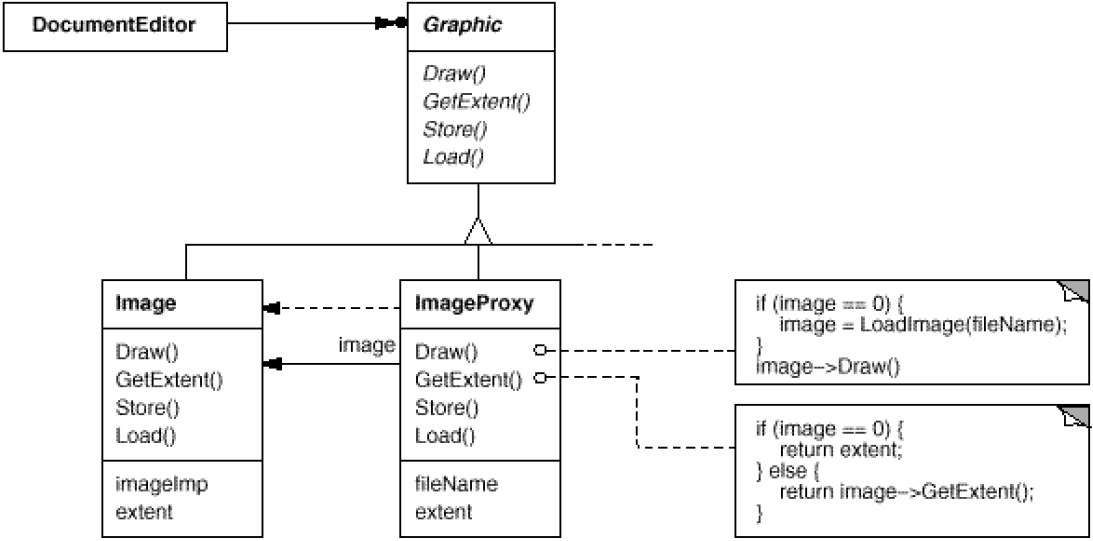
\includegraphics[width=\linewidth]{/proxy}
\subsubsection{Beschreibung}
Provide a surrogate or placeholder for another object to control access to it.\\
Bietet einen Stellvertreter oder Platzhalter für ein anderes Objekt. Ein Proxy kontrolliert den Zugrff auf das originial Objekt, was erlaubt vor oder nach dem eigentlichen Request, Code auszuführen.
\subsubsection{Vorteile}
\begin{itemize}[topsep=0pt]
    \itemsep -0.4em
    \item Das Service Objekt kann kontrolliert werden, ohne dass der Client etwas davon weiss
    \item Ermöglicht das Managen des Life-Cycles des Services, wenn sich Clients nicht darum kümmern
    \item Proxy funktioniert auch, wenn der Service nicht ready oder nicht verfügbar ist
    \item Open/Closed Principle: Neue Proxies können erstellt werden, ohne den Service oder Client zu verändern
\end{itemize}
\subsubsection{Nachteile}
\begin{itemize}[topsep=0pt]
    \itemsep -0.4em
    \item Code kann komplizierter werden, da neue Klassen erstellt werden müssen
    \item Antwort des Services kann verzögert werden
\end{itemize}
\subsubsection{Eigene Notizen}
\textbf{Identifikation:} Delegieren die eigentliche Arbeit an andere Objekte. Jede Proxy-Methode soll zu einem Service-Objekt referenzieren\\
\textbf{Anwendung:} Wird sehr oft verwendet, wenn zusätzlicher Code ausgeführt werden soll

\subsection{Facade (Structural)}
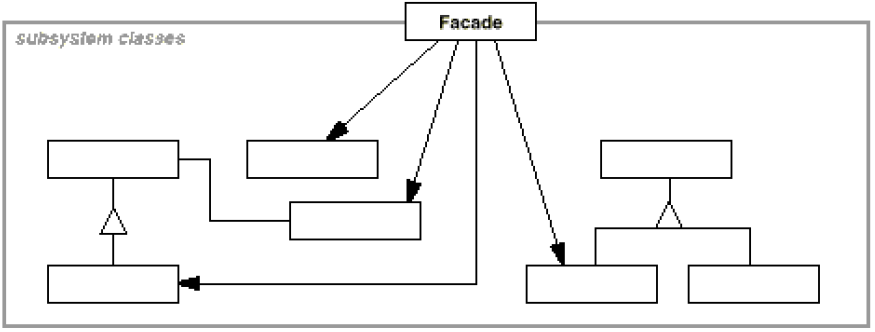
\includegraphics[width=\linewidth]{/facade}
\subsubsection{Problem}

\subsubsection{Beschreibung}
Provide a unified interface to a set of interfaces in a subsystem. Facade defines a higher-level interface that makes the subsystem easier to use.\\
Subsysteme können Libraries, Frameworks oder ein komplexes Set von Klassen sein.
\subsubsection{Vorteile}
\begin{itemize}[topsep=0pt]
    \itemsep -0.4em
    \itemDer Code kann von der Komplexität des Subsystems isoliert werden
\end{itemize}
\subsubsection{Nachteile}
\begin{itemize}[topsep=0pt]
    \itemsep -0.4em
    \item Facade kann ein God-Object, welches an alle Klassen einer App gekoppelt ist werden
\end{itemize}
\subsubsection{Eigene Notizen}

\textbf{Identifikation:} Ist meistens eine Klasse mit einer einfachen Schnittstelle, welche aber alle Arbeit an andere Klassen weiter delegiert. Facade managen oftmals den Life-Cycle der Objekte die sie verwendet.\\
\textbf{Auftreten:} Passiert sehr viel innerhalb einer einfachen Schnittstelle


%Behavioral
\subsection{Observer (Behavioral)}
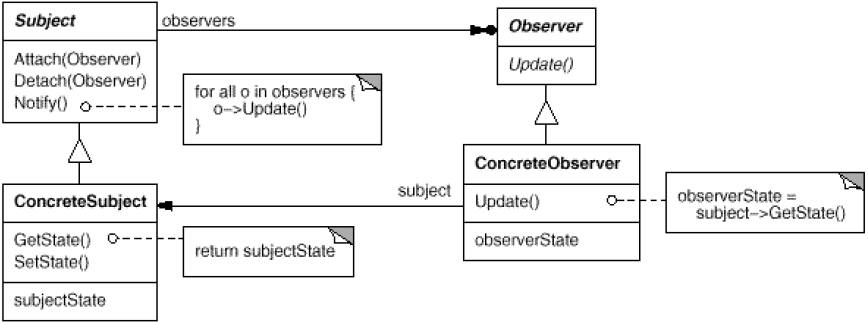
\includegraphics[width=\linewidth]{observer}
\subsubsection{Problem}
Anstelle, dass Objekt A beim Objekt B regelmässig abfragt, ob es sich geändert hat, benachrichtigt B A, dass es sich geändert hat. Benachrichtige mich wenn.. $\rightarrow$ Subject informiert alle Observer
\subsubsection{Beschreibung}
Define a one-to-many dependency between objects so that when one object changes state, all its dependents are notified and updated automatically.
\subsubsection{Vorteile}
\begin{itemize}[topsep=0pt]
    \itemsep -0.4em
    \item Open/Closed Prinzip: Es können neue Subscriber Klassen erstellt werden, ohne den Publisher ändern zu müssen
    \item Es können zur Laufzeit beziehungen zwischen Objekten erstellt werden
\end{itemize}
\subsubsection{Nachteile}
\begin{itemize}[topsep=0pt]
    \itemsep -0.4em
    \item Subscribers werden in zufälliger Reihenfolge benachrichtigt
\end{itemize}
\subsubsection{Eigene Notizen}
\textbf{Identifikation:} Hat Subscription Methoden, die Objekte in einer Liste speichert und eine Update Methode für diese Objekte ausführt.\\
\textbf{Beispiel:} Click Event Handlers im Web

\subsection{Strategy (Behavioral)}
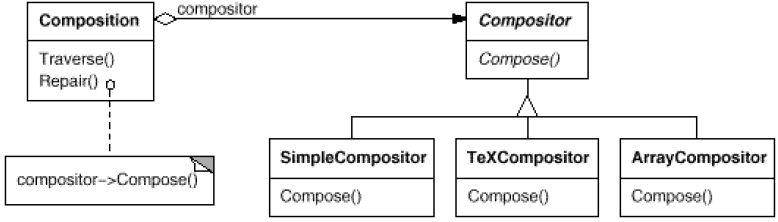
\includegraphics[width=\linewidth]{/strategy}
\subsubsection{Problem}
Verschiedene Compositors (Algorithmen) anbieten. Das Objekt Composition verwendet dann denn benötigten Compositor.
\subsubsection{Beschreibung}
Define a family of algorithms, encapsulate each one, and make them interchangeable. Strategy lets the algorithm vary independently from clients that use it.
\subsubsection{Vorteile}
\begin{itemize}[topsep=0pt]
    \itemsep -0.4em
    \item Algorithmen können zur Laufzeit ausgetauscht werden (Polymorphie)
    \item Isolation der Implementations Details (Algorithmen) gegenüber dem Code, welcher sie verwendet
    \item Vererbung kann mit Composition ausgetauscht werden
    \item Open/Close Principle: Es können neue Strategien hinzugefügt werden, ohne den Kontext zu ändern
\end{itemize}
\subsubsection{Nachteile}
\begin{itemize}[topsep=0pt]
    \itemsep -0.4em
    \item Überkompliziert, wenn nur wenige Algorithmen existieren und diese selten ausgetauscht werden
    \item Clients müssen die unterschiede der Algorithmen kennen, damit der richtige ausgewählt werden kann
\end{itemize}
\subsubsection{Eigene Notizen}
\textbf{Umsetzung mit:} Factory Method, oder beim Erstellen dem Konstruktor übergeben.\\
\textbf{Identifikation:} Hat eine Methode, die nested Objekte die Arbeit machen lässt und einen Setter, damit das Objekt ausgetauscht werden kann.\\
\textbf{Beispiel:} Unterschiedliche Algorithmen für einen Routen planer.

\subsection{Template Method (Behavioral)}
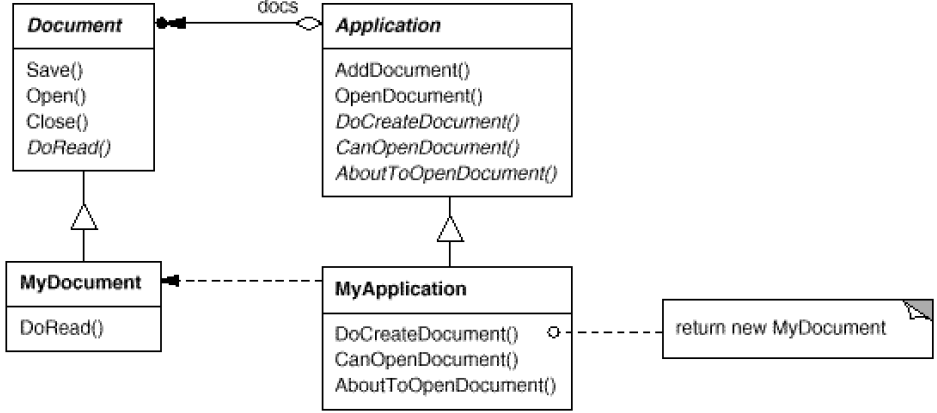
\includegraphics[width=\linewidth]{/template_method}
\subsubsection{Problem}
Austauschen einzelner Schritte eines Workflows.
\subsubsection{Beschreibung}
Define the skeleton of an algorithm in an operation, deferring some steps to subclasses. Template Method lets subclasses redefine certain steps of an algorithm without changing the algorithm's structure.
\subsubsection{Vorteile}
\begin{itemize}[topsep=0pt]
    \itemsep -0.4em
    \item Clients können Teile eines Algorithmus austauschen
    \item Duplizierter Code kann in Super-Klasse verschoben werden
\end{itemize}
\subsubsection{Nachteile}
\begin{itemize}[topsep=0pt]
    \itemsep -0.4em
    \item Klassen können durch das bereitgestellte Gerüst limitiert werden
    \item Das Likov Substitution Principle kann verletzt werden, indem keine Default-Implementierung möglich ist
    \item Template Methoden werden schwerer unterhalten, je mehr schritte existieren
\end{itemize}
\subsubsection{Eigene Notizen}
\textbf{Identifikation:} Haben Verhaltens-Methoden, die ein \dq default\dq-Verhalten in der Basis-Klasse implementiert haben\\
\textbf{Application:} Die Funktionen der Application können bereits das Patterns Factory Method implementieren. z.B. Beinhaltet die Funktion AddDocument() die Abstrakte Klasse DoCreateDocument()

\subsection{Mediator (Vermittler) (Behavioral)}
\subsubsection{Beschreibung}
Reduziert chaotische Abhängigkeiten zwischen Objekten. Das Pattern verhindert direkte Kommunikation zwischen den Objekten und zwingt diese mit dem Madiator-Objekt zusammenzuarbeiten.
\subsubsection{Problem}
\begin{itemize}[topsep=0pt]
    \itemsep -0.4em
    \item Object Structures may result in many connections between objects
    \item In the worst case, every object ends up knowing about every other
\end{itemize}
\textbf{Intent:}
\begin{itemize}[topsep=0pt]
    \itemsep -0.4em
    \item How can strong coupling between multiple objects be avoided and communication simplified?
\end{itemize}
\subsubsection{Solution}
Define an object that encapsulates how a set of objects interact. Mediator promotes loose coupling by keeping objects from referring to each other explicitly, and lets you vary their interaction independently.\\ 
\textbf{Mediator:} Encapsulates how a set of objects interact\\ 
\textbf{Colleaues:} Refer to Mediator; this promotes loose coupling\\ 
\textbf{Static Structure:}\\
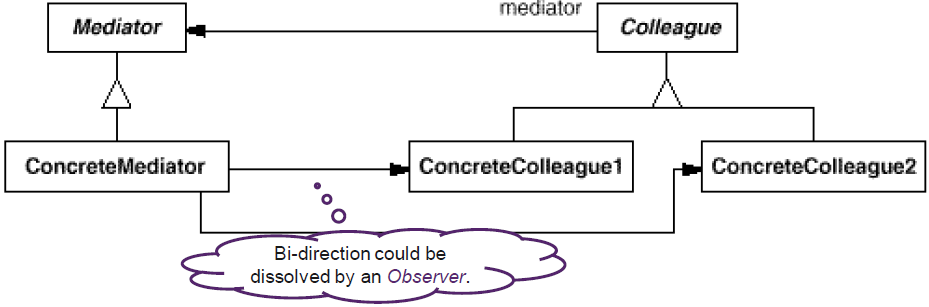
\includegraphics[width=\linewidth]{/mediator_static}
\textbf{Dynamics:}\\ 
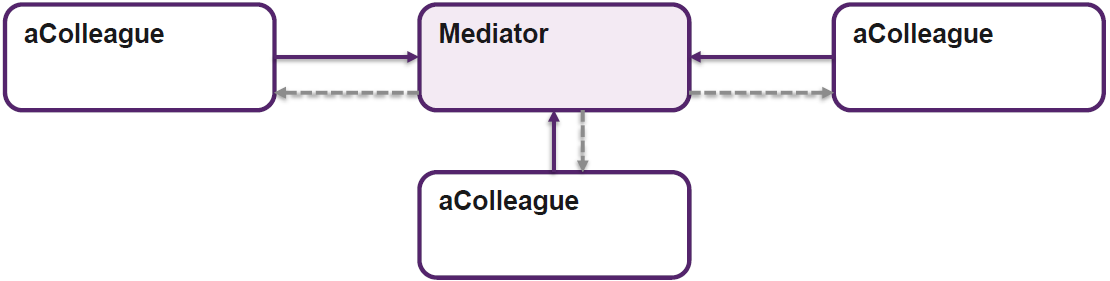
\includegraphics[width=\linewidth]{/mediator_dynamic}
\subsubsection{Implementation}
\begin{itemize}[topsep=0pt]
    \itemsep -0.4em
    \item Mediator as an Observer
    \item Colleagues act as Subject
\end{itemize}
\textbf{Known Uses:}
\begin{itemize}[topsep=0pt]
    \itemsep -0.4em
    \item Message Bus Systems
    \item Redux Dispatcher
\end{itemize}
\subsubsection{Vorteile}
\begin{itemize}[topsep=0pt]
    \itemsep -0.4em
    \item Colleague classes may become more reusable, low coupling
    \item Centralizes control of communication between objects
    \item Encapsulates protocols
    \item Single Responsibility Principle: Kommunikation zwischen verschiedenen Komponenten kann zu einem Ort extrahiert werden. Macht es einfacher diese zu Unterhalten
    \item Open/Closed Principle Es können neue Mediators hinzugefügt werden, ohne die Komponenten zu ändern
    \item Reduziert die Kopplung zwischen den Komponenten
    \item Individuelle Komponenten können einfacher wiederverwenet werden
\end{itemize}
\subsubsection{Nachteile:}
\begin{itemize}[topsep=0pt]
    \itemsep -0.4em
    \item Adds complexity
    \item Single point of failure
    \item Limits subclassing (of mediator class)
    \item May result in hard maintainable monoliths
    \item Mediator kann zu einer God-Klasse werden
\end{itemize}
\subsubsection{Eigene Notizen}
Der Controller-Teil von MVC ist ein Synonym für Mediator
\textbf{Teilnehmer:} Mediator, Colleague

\subsection{Memento (Behavioral)}
\subsubsection{Beschreibung}
Erlaubt das Speichern und Wiederherstellen von vorherigen Zuständen eines Objekts, ohne die Implementierungs Details zu enthüllen
\subsubsection{Problem}
\begin{itemize}[topsep=0pt]
    \itemsep -0.4em
    \item Sometimes it's necessary to record the internal state of an object
    \item Objects normally encapsulate their state, making it inaccessible
\end{itemize}
\textbf{Intent:}
\begin{itemize}[topsep=0pt]
    \itemsep -0.4em
    \item How can the state of an object be externalized without violating its encapsulation?
\end{itemize}
\subsubsection{Solution}
Without violating encapsulation, capture and externalize an objects internal state so that the object can be restored to this state later.\\
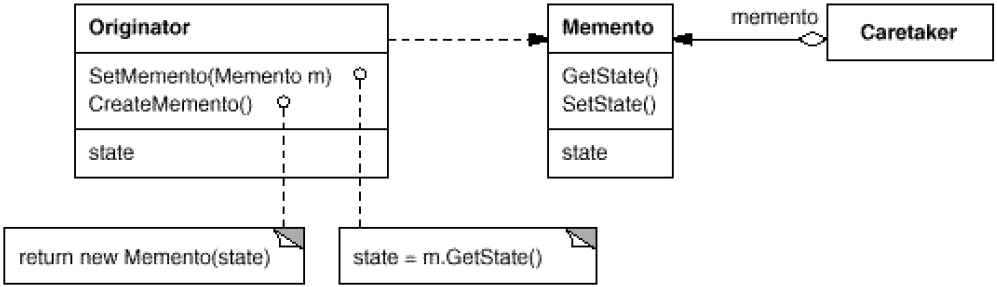
\includegraphics[width=\linewidth]{/memento}
\textbf{Dynamics:}\\ 
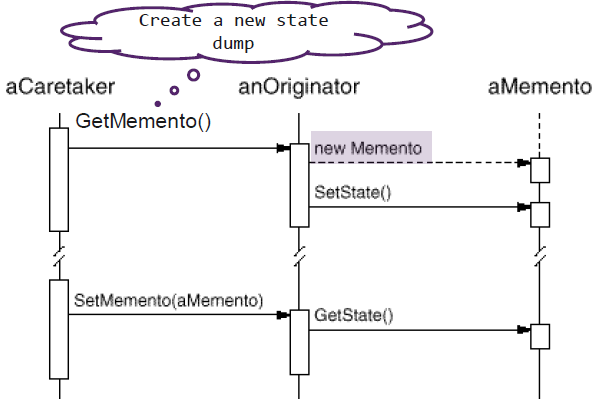
\includegraphics[width=0.7\linewidth]{/memento_dynamic}

\subsubsection{Participants}
\textbf{Memento}
\begin{itemize}[topsep=0pt]
    \itemsep -0.4em
    \item Stores some/all the internal state of the Originator
    \item Allows only the originator to access its internal information
\end{itemize}
\textbf{Originator}
\begin{itemize}[topsep=0pt]
    \itemsep -0.4em
    \item Can create Memento objects to store its internal state at strategic points
    \item Can restore own state to what the Memento object dictates
\end{itemize}
\textbf{Caretaker}
\begin{itemize}[topsep=0pt]
    \itemsep -0.4em
    \item Stores the Memento objects
    \item Cannot explore/operate the contents
\end{itemize}
\subsubsection{Implementation}
\begin{itemize}[topsep=0pt]
    \itemsep -0.4em
    \item Originator creates memento and passes over its internal state
    \item Can be combined with Factory Method
    \item Declare Originator as \textit{friend} of Memento, so Originator can read out its properties
\end{itemize}
\subsubsection{Vorteile}
\begin{itemize}[topsep=0pt]
    \itemsep -0.4em
    \item Internal State of an object (snapshots) can be saved and restored at any time
    \item Encapsulation of attributes is not harmed
    \item State of objects can be restored later
    \item Originator Code kann vereinfacht werden, indem der Caretaker Rücksicht auf die History des Originator Zustandes nimmt
\end{itemize}
\subsubsection{Nachteile}
\begin{itemize}[topsep=0pt]
    \itemsep -0.4em
    \item Creates a complete copy of the object every time, no diffs (memory usage)
    \item No direct access to saved state, it must be restored first
    \item App kann sehr viel RAM brauchen
    \item Caretakers müssen den Life-Cycle des Originator verfolgen, damit überflüssige Mementos gelöscht werden können
\end{itemize}
\subsubsection{Eigene Notizen}
\begin{itemize}[topsep=0pt]
    \itemsep -0.4em
    \item Ohne Memento müsten die Felder einer Klasse public sein
    \item Moderne Alternativen sind Serialisierung (Java/C\#). Sei es Serialisierung für eine Datenbank, oder ein File-System. Ähnlich zu Future-Token
    \item Wird in Java oftmals mit Serializable gemacht
    \item Teilnehmer: Memento, Originator, Caretaker
\end{itemize}

\subsection{Command (Behavioral)}
\subsubsection{Beschreibung}
Wandelt einen Request in ein stand-alone Objekt um, welches alle Informationen zum Request enthaltet. Das erlaubt, dass Requests als Methoden-Argumente verwendet werden, die Request verzögert werden, in einer Warteschlange stehen und erlaubt undoable operationen.
\subsubsection{Problem}
\begin{itemize}[topsep=0pt]
    \itemsep -0.4em
    \item Decouple the decision of what to execute from the decision of when to execute
    \item The execution needs an additional parametrization context
\end{itemize}
\textbf{Intent:}
\begin{itemize}[topsep=0pt]
    \itemsep -0.4em
    \item How can commands be encapsulated, so that they can be parameterized, scheduled, logged and/or undone?
\end{itemize}
\subsubsection{Solution}
Encapsulate a request as an object, thereby letting you parameterize clients with different requests, queue or log requests, and support undoable operation.\\ 
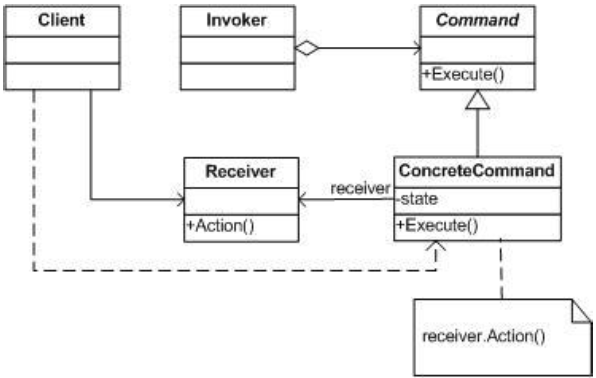
\includegraphics[width=\linewidth]{/command}
\textbf{Dynamics:}\\ 
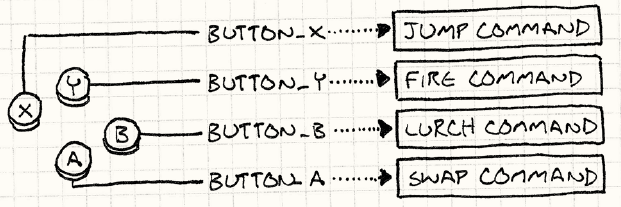
\includegraphics[width=\linewidth]{/command_dynamic}
\subsubsection{Vorteile}
\begin{itemize}[topsep=0pt]
    \itemsep -0.4em
    \item The same command can be activated from different objects
    \item New commands can be introduced quickly and easily
    \item Command objects can be saved in a command history
    \item Provides inversion of control, encourages decoupling in both time and space
    \item Single Responsibility Principle: Klassen die Operationen aufrufen, können von den Klassen die Operationen ausführen, entkoppelt werden
    \item Open/Closed Principle: Neu Commandos können hinzugefügt werden ohne existierenden Client Code zu zerstören
    \item Undo/Redo kann implementiert werden
    \item Das Ausführen von Operationen kann aufgeschoben werden
    \item Ein Set von einfachen Commands kann zu einem komplexen zusammengestellt werden
\end{itemize}
\subsubsection{Nachteile}
\begin{itemize}[topsep=0pt]
    \itemsep -0.4em
    \item Large designs with many commands can introduce many small command classes mauling the design
    \item Der Code kann komplizierter werden, weil ein neues Layer zwischen Sender und Empfänger hinzugefügt wird
\end{itemize}
\subsubsection{Eigene Notizen}
\textbf{Identfikation:} Wenn es ein Set von ähnlichen Klassen hat, welche spezifische Aktionen darstellen (Copy, Cut, Send, Print etc.). Diese Klassen sollten das selbe Interface implementieren. Zusätzlich hat es meistens eine Klasse, welche diese Aktionen als Argument akzeptiert
\begin{itemize}[topsep=0pt]
    \itemsep -0.4em
    \item Do und Undo werden im Command gespeichert
    \item Wird z.B. verwendet für callbacks, Queueing Tasks, Tracking Operations History etc.
\end{itemize}

\subsection{Command Processor (Behavioral)}
\subsubsection{Beschreibung}
Separiere den Request für einen Service von dessen Ausführung. Command Processor Komponente verwaltet Requests als separate Objekte, plant zeitlich dessen Ausführung und bietet zusätzliche Services, wie das Speichern von Request-Objekten für späters undo.
\subsubsection{Problem}
\begin{itemize}[topsep=0pt]
    \itemsep -0.4em
    \item Common UI applications support do and multiple undo steps
    \item Steps forward and backward are accessible in a history
\end{itemize}
\textbf{Intent:}
\begin{itemize}
    \item How could we manage command objects, so the execution is seperated from the request and the execution can be undone later?
\end{itemize}
\subsubsection{Solution}
Separate the request for a service from its execution. A command processor component manages requests as separate objects, schedules their execution, and provides additional services such as the storing of request objects for later undo.\\ 
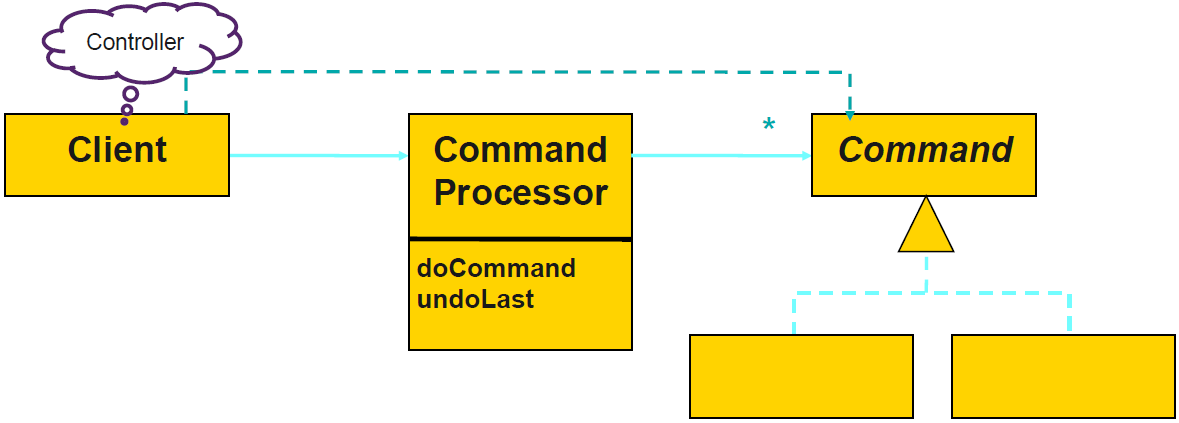
\includegraphics[width=0.8\linewidth]{/command_processor}
\textbf{Dynamics:}\\ 
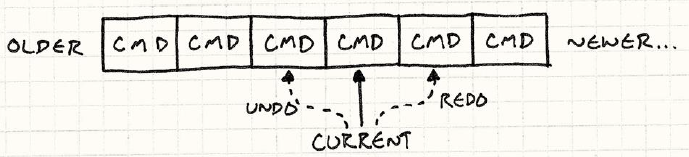
\includegraphics[width=\linewidth]{/command_processor_dynamic}
\subsubsection{Participants}
\textbf{Command Processor}
\begin{itemize}[topsep=0pt]
    \itemsep -0.4em
    \item A Separate processor object can handle the responsibility for multiple Command objects
\end{itemize}
\textbf{Command}
\begin{itemize}[topsep=0pt]
    \itemsep -0.4em
    \item A uniform interface to execute functions
\end{itemize}
\textbf{Controller}
\begin{itemize}[topsep=0pt]
    \itemsep -0.4em
    \item Translates requests into commands and transfers commands to Command Processor.
\end{itemize}
\subsubsection{Implementation}
\begin{itemize}[topsep=0pt]
    \itemsep -0.4em
    \item Command Processor contains a \textit{Stack} which holds the command history
    \item Controller creates the Commands and passes them over to Command Processor
    \item Creation of Commands may be delegated to a \textit{Simple Factory}
\end{itemize}
\subsubsection{Vorteile}
\begin{itemize}[topsep=0pt]
    \itemsep -0.4em
    \item Flexibility $\rightarrow$ Command Processor und Controller werden unabhängig von Commands implementiert
    \item Allows addition of services related to command execution
    \item Enhances testability $\rightarrow$ Command Processor kann verwendet werden, um Regression Tests durchzuführen
\end{itemize}
\subsubsection{Nachteile}
\begin{itemize}[topsep=0pt]
    \itemsep -0.4em
    \item Efficiency loss due additional indirection
\end{itemize}
\subsubsection{Eigene Notizen}
\begin{itemize}
    \item Dank dem Command Processor Pattern kann z.B. ein Logger eingeführt werden, dies ist nur mit dem Command nicht möglich! Command ist nur ein Interface!
    \item Teilnehmer: Command Processor, Command, Controller
\end{itemize}

\subsection{Visitor (Behavioral)}
\subsubsection{Beschreibung}
Erlaubt das Ausführen einer Operation auf den Elementen einer Objekt Struktur. Ermöglicht den Algorithmus vom Objekt zu separieren, auf dem es ausgeführt wird.
\subsubsection{Problem}
\begin{itemize}[topsep=0pt]
    \itemsep -0.4em
    \item Operations on specific classes needs to be changed/added without needing to modify these classes
    \item Different algorithms needed to process an object tree
\end{itemize}
\textbf{Intent:}
\begin{itemize}[topsep=0pt]
    \itemsep -0.4em
    \item How can the behaviour on individual elements of a data structure be changed/replaced whout changing the elements?
\end{itemize}
\subsubsection{Solution}
Represent an operation to be performed on the elements of an object structure. Visitor lets you define a new operation without changing the classes of the elements on which it operates.\\ 
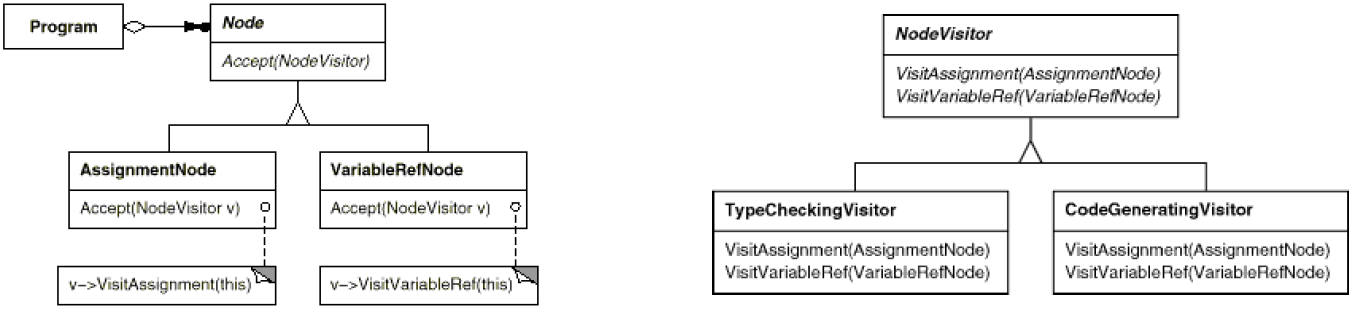
\includegraphics[width=\linewidth]{visitor}
\subsubsection{Implementation}
\begin{itemize}[topsep=0pt]
    \itemsep -0.4em
    \item 2 Class Hierarchies (Elements / Visitors)
    \item Visitors iterate though object hierarchy
    \item Solves Double-Dispatch problem of single dispatched programming languages
\end{itemize}
\textbf{Patterns that combine naturally with Vistor:}
\begin{itemize}[topsep=0pt]
    \itemsep -0.4em
    \item Composite
    \item Interpreter
    \item Chain of Responsibility
\end{itemize}
\subsubsection{Vorteile}
\begin{itemize}[topsep=0pt]
    \itemsep -0.4em
    \item Visitor makes adding new operatios easy
    \item Separates related operations from unrelated ones
    \item Open/Closed Principle: Neues Verhalten, welches auf Objekten unterschiedlicher Klassen ausgeführt werden kann, ohne die Klassen zu ändern
    \item Single Responsibility Principle: Mehrere Versionen des selben Verhaltens können in die selbe Klasse verschoben werden
    \item Es können komplexe Datenstrukturen traversiert werden
\end{itemize}
\subsubsection{Nachteile}
\begin{itemize}[topsep=0pt]
    \itemsep -0.4em
    \item Adding new node classes is hard
    \item Visiting sequence is fix defined within nodes
    \item Visitor breaks logic apart
    \item Alle Visitors müssen geupdatet werden, wenn eine Klasse hinzugefügt oder entfernt wird
    \item Visitors können nicht auf private Felder zugreifen
    \item Schlecht wenn die Klassen-Hierarchie sich ändert
\end{itemize}
\subsubsection{Eigene Notizen}
\begin{itemize}[topsep=0pt]
    \itemsep -0.4em
    \item Wenn unterschiedliche Algorithmen verwendet werden, um ein Object-Tree zu verarbeiten
    \item Visitor werden sehr oft mit Composite, Interpreter oder Chain of Responsibility kombiniert
\end{itemize}